% This is the aspauthor.tex LaTeX file
% Copyright 2010, Astronomical Society of the Pacific Conference Series

\documentclass[11pt,twoside]{article}
\usepackage{asp2010}
\usepackage{epstopdf}


\resetcounters

%\bibliographystyle{asp2010}

\markboth{Christophe Arviset, Deborah Baines, and Pedro Osuna}{C.Arviset et al}

\begin{document}

\title{Results from the Survey of ESA Science Archives}
\author{Christophe~Arviset$^1$, Deborah~Baines$^1$, and Pedro~Osuna$^1$
\affil{$^1$ESA-ESAC, POBOX 78, 28691 Villanueva de la Canada, Madrid, Spain}}

\begin{abstract}
Most of ESA's Space Science Archives are currently hosted at ESAC, the European Space Astronomy Centre, located near Madrid, Spain. All these science archives are designed, developed, operated and maintained by a dedicated Science Archives and VO Team, providing support to all science operations centres at ESAC. At the end of 2011, a questionnaire was sent to all users of the ESAC Science Archives in the last five years, asking them about their usage frequency, their satisfaction level, the type of interfaces used (GUI or scriptable interface or others) and the purpose for which they are using the archives. The survey also allowed optionally to provide qualitative feedback. This paper presents the main results from this questionnaire, from a global perspective of all the archives.
\end{abstract}

\section{Science Archives at ESAC}
Over the years, ESAC has turned into a Science Data Centre, hosting most of ESA Space Science astronomy and solar system missions' archives (Figure~\ref{P02_f1_Archives}) . This includes active archives for which new data are being ingested regularly, such as the XMM-Newton Science Archive (XSA), the Herschel Science Archive (HSA), the Integral SOC Science Data Archive (ISDA), the SOHO Science Archive (SSA), ESA's Planetary Science Archive (the PSA with Mars Express, Venus Express and Rosetta), the Planck Legacy Archive (PLA) and more recently in 2012, the European HST Archive. Furthermore, support for legacy archives is also provided, such as for the ISO Data Archive (IDA), the EXOSAT Science Archive (EXSA) and legacy planetary missions within the PSA (SMART-1, Huygens and Giotto). Cluster and Ulysses final archives are being migrated to ESAC and development is starting for upcoming missions such as Gaia, Euclid, Solar Orbiter and BepiColombo.

The ESAC Science Archives provide complementary services to different types of users, primarily towards scientists to enable maximum scientific exploitation of data sets, but as well to science operations teams through cost-effective archive production by integration in, and across, projects. Furthermore, science archives must ensure efficient long-term preservation of data, software and knowledge for several decades, well after the mission lifetime itself, with sufficient flexibility to adapt to modern technology.

The Standard access to the archives is through powerful web based GUI interfaces (http://archives.esac.esa.int/), offering simple to use, powerful search and results facilities, handling of proprietary and public data, direct download, shopping basket, on the fly reprocessing (for some archives), links (back and forth) to the science literature and interoperability with external VO Tools. Additionally, there are scriptable Archive Machine Interfaces which can be easily coupled with GRID to batch data access for further processing. These are mainly used by Science Operations Teams at ESAC and by the instrument teams for calibration and trend analysis purposes. These can also be used for systematic data processing by some projects (e.g. Herschel) or external mirror sites.


\begin{figure}[t]
\begin{center}
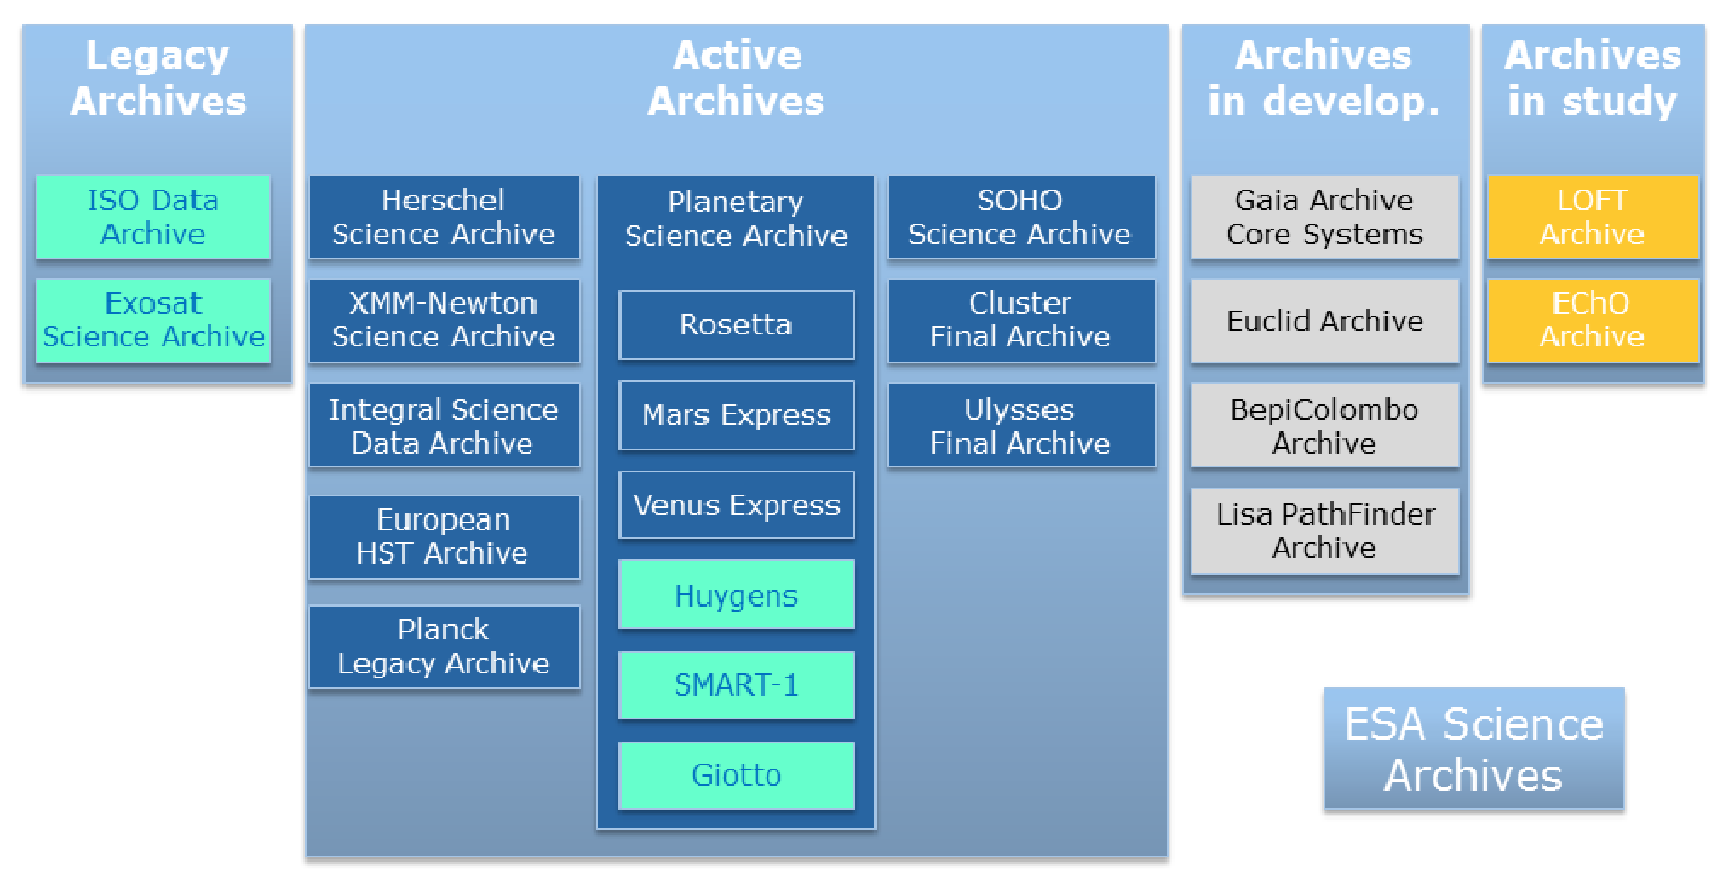
\includegraphics[width=1.0\hsize]{P02_f1-Archives.eps}
\caption{ESA Science Archives and associated phases} \label{P02_f1_Archives}
\end{center}
\end{figure}

\section{Results from the Survey of ESAC Science Archives}

\subsection{The Questionnaire}
The questionnaire consists of a web based form, open for five weeks at the end of 2011. It was designed to only take a user a few minutes to answer. The first five questions were compulsory, with options as radio buttons and tick boxes about the following:
\begin{itemize}
\checklistitemize
\item which archives are being used, 
\item the satisfaction level, 
\item the type of archive interface mainly used (web GUI, scriptable interface, map based, or others depending on the archive), 
\item the purpose of usage (science research, mission support, others) and 
\item the way of using the archives (browsing data, downloading different types of data, preparing observing proposals, others).
\end{itemize}
Furthermore, there were four more questions allowing users to provide qualitative feedback about what they like the most and the least about the archives, suggestions for additional features or any other comments.

The questionnaire was announced to all users who have used one of the ESAC Science Archives in the last five years, as well as announced via the projects newletters. In total, we estimate that it has been sent to around 4500 users. 385 responses have been received, representing a good response rate of 8.4\% which enabled a good statistical basis for a proper analysis of the results.

\subsection{The Quantitative Results}
The quantitative results are presented in Figure~\ref{P02_f2_Results}. Over a third of the users are using the archives daily (9\%) or a few times a week (27\%) while another third (38\%) use them a few times per month. The remaining part (26\%) are using them only a few times a year or even less.

The wide majority of the users are using the archives for scientific research (69\%), which confirms the purpose of the ESAC archives to primarily serve the scientific community to enhance the science return from ESA Science missions. The second objective is met with serving the mission teams (16\%), such as the Science Operations Centres and instrument teams. We note the other types of usage such as Education and Outreach (10\%) and Amateur Astronomy (4\%), which can go over 40\% for the Soho Science Archive, extensively used for discovering comets.

The main purpose in using the Archives is for downloading public data and browsing for data (23\% and 22\% respectively). Preparing observing proposals and downloading proprietary data are both at 16\%, downloading science-ready data products are at 14\%, identifying areas with sufficient coverage for science projects is at 8\%, and 1\% of the users said they use Archives for other purposes.

The web interface remains the preferred option for users to access the archives (80\%), whereas the machine scriptable interface requires more expertise and is used by 9\% of them. Other interfaces dedicated for some archives are also used by 8\% for HIPE from the Herschel Science Archive, and 2\% for the Dataset Browser and 1\% for the Mars Map Browser, both from the Planetary Science Archive.

Overall, the results on the satisfaction with the Archives is very positive, with 22\% of users very satisfied, 41\% are satisfied, 30\% are neutral, 5\% are dissatisfied and 2\% very dissatisfied. The high percentage of neutral response might be due to the way the questions were asked, in the sense that satisfaction level was required to be given for all individual archives, although users usually do not use them all. The ratio of (very satisfied + satisfied)/(dissatisfied + very dissatisfied) = 9. In some cases the ratio for individual Archives is considerably higher, such as the XMM-Newton Science Archive (ratio of $\sim$23) and the Soho Science Archive (ratio of $\sim$18). 

It is also worth noting the intensive use of a legacy archive, such as the ISO Data Archive. As can be seen in the report, the ISO Data Archive is being used extensively, and we find a correlation of its usage with the usage of the Herschel Science Archive, which makes sense, as legacy archives of a determined wavelength range can be used for preparation of new observations in operational missions in the same wavelength range. This enhances the necessity and convenience of the Long Term preservation of ESA missions� archival data, and supports the approach taken at ESAC where the infrastructure for Science Archives allows for a low cost maintenance and operation of legacy archives.

\begin{figure}[t]
\begin{center}
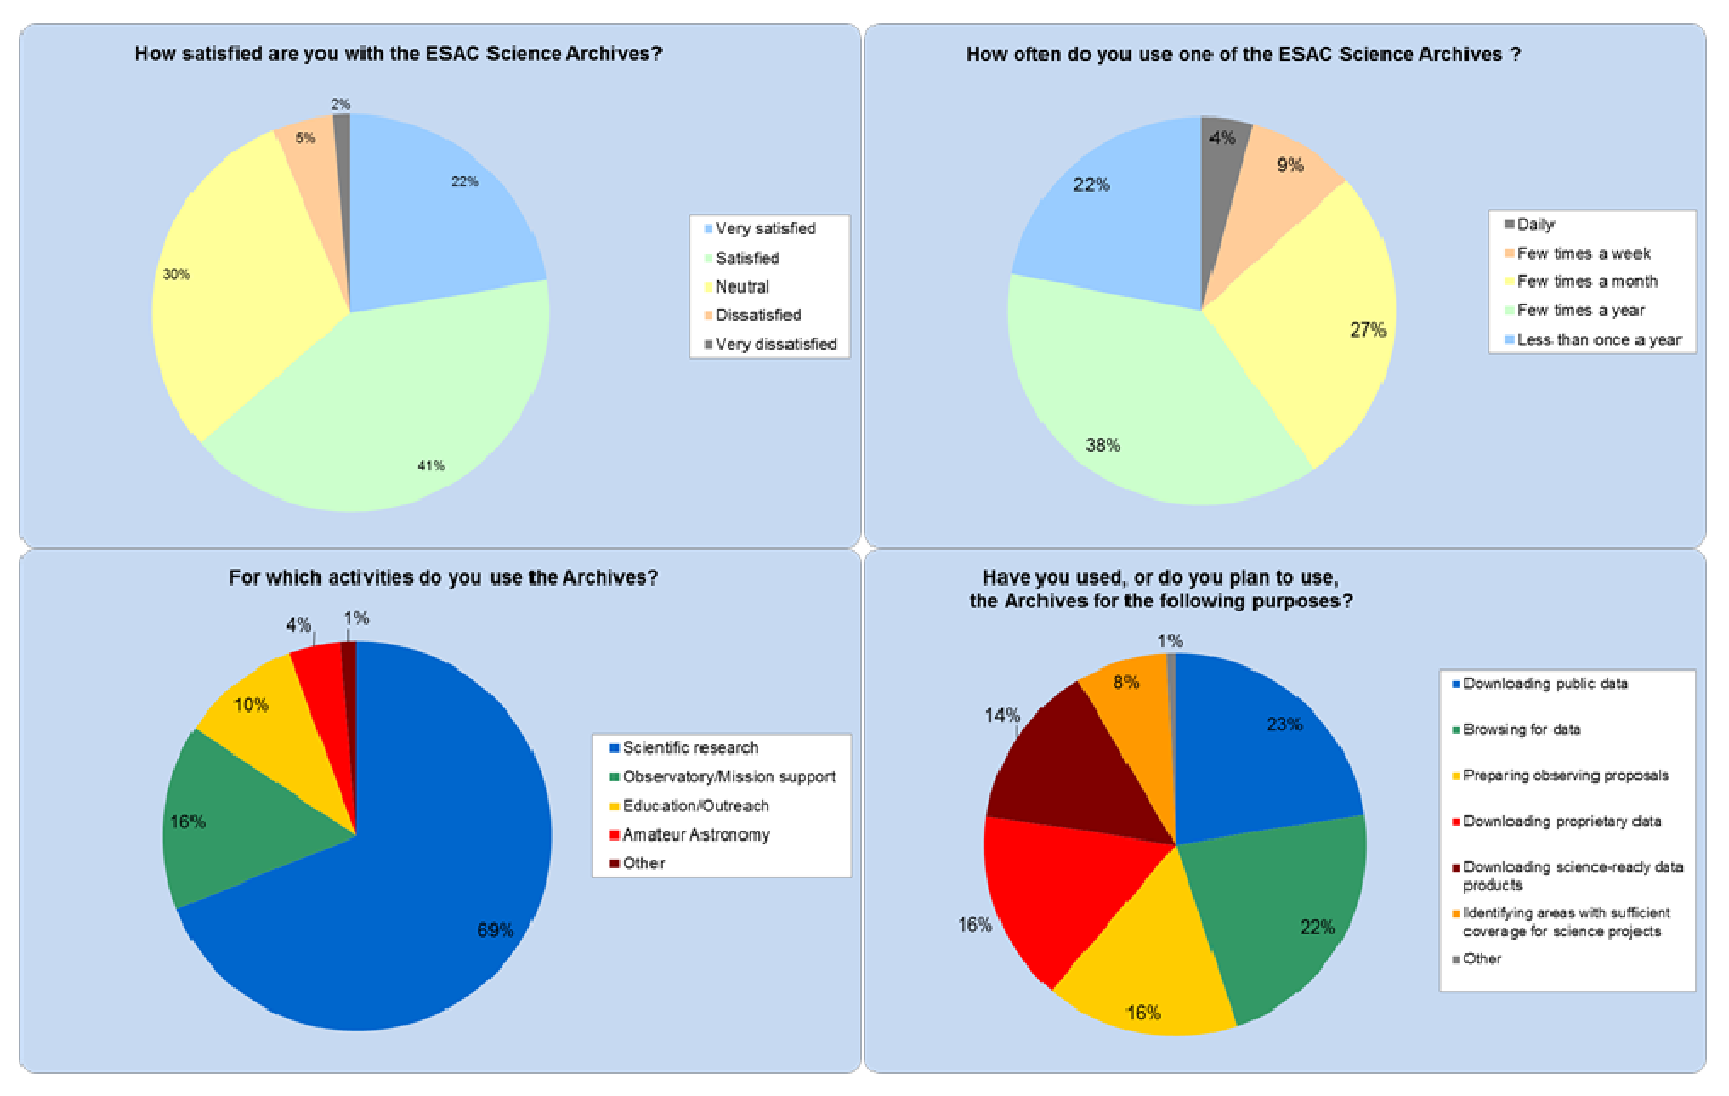
\includegraphics[width=1.0\hsize]{P02_f1-SurveyResults.eps}
\caption{The Quantitative Survey Results} \label{P02_f2_Results}
\end{center}
\end{figure}

\subsection{The Qualitative Results}
The questionnaire offered the possibility for users to provide feedback in a more free text form. Over 250 individual comments were received and have been arranged into the following categories: interfaces (feedback related to the Archive�s Interfaces), technology (feedback related to the current technology used in the Archives, or on possible future technologies), data (feedback related to the data contained within the Archives), support (feedback related to the user and technical support provided by the Archives), and then feedback on any other topics.

The majority of feedback received was on the topic of the Archives Interfaces where the most common subjects discussed were the following: ease of use and layout of the graphical user interface, simple and advanced search options, query results and download options, common look and feel to the Archives, web interface versus Java (rich client) interface, and the archive scriptable machine interface.

The analysis of these comments (sometimes contradictory!) confirms the wide variety of users accessing the archives for different purposes and needs. Overall, these will enable an improvement in the quality of the services offered by the ESAC Science Archives to their user communities.


\section{Conclusion}
Making a survey of ESAC Science Archives has revealed to be a very useful exercise to understand better the expectations of our users, the way they are using our services and their associated level of satisfaction. It has provided information that will enable us to continuously improve our services in order to increase the science return from ESA science missions. 

\acknowledgements The authors would like to thank the ESAC Science Archives Team as well as the Archive Scientists for each of the science archives at ESAC.


%\bibliography{aspauthor}

\end{document}
